\documentclass[tikz,border=3pt]{standalone}
\usepackage{amsmath}
\usepackage{tikz}
\usepackage{pgfplots}
\pgfplotsset{compat=1.18}
\begin{document}
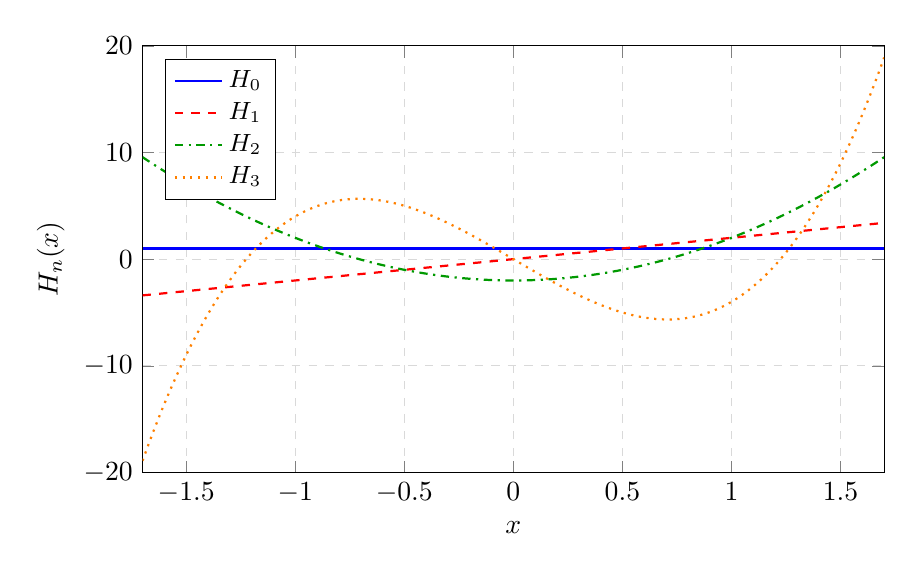
\begin{tikzpicture}
\begin{axis}[
  width=11cm, height=7cm,
  xlabel=$x$, ylabel={$H_n(x)$},
  xmin=-1.7, xmax=1.7, ymin=-20, ymax=20,
  legend style={at={(0.03,0.97)}, anchor=north west, font=\small},
  grid=both, grid style={dashed, gray!30},
  domain=-1.7:1.7, samples=200,
  no marks
]
  \addplot[blue, thick, solid]           {1};
  \addlegendentry{$H_0$}
  \addplot[red, thick, dashed]            {2*x};
  \addlegendentry{$H_1$}
  \addplot[green!60!black, thick, dashdotted] {4*x^2 - 2};
  \addlegendentry{$H_2$}
  \addplot[orange, thick, dotted]         {8*x^3 - 12*x};
  \addlegendentry{$H_3$}
\end{axis}
\end{tikzpicture}
\end{document}
